\chapter{Situational \& Theoretical Analysis}\label{chap:situational_theoretical_analysis}

\section{Thread Wireless Network}\label{sec:thread_wireless_network}
Thread wireless network, introduced in 2014, is an open standard designed for secure, low-power, and cost-effective IPv6 communication in connected home and commercial applications. Thread offers simple installation, self-configuring, dynamic optimization, and self-healing capabilities, utilizing a low-power wireless mesh network topology, which ensures scalability and reliability \cite{Thread_Group_Benefits}. Its low power consumption makes it ideal for smart home devices running on batteries and supports long-range communication. Thread uses IPv6 security features and Backbone Border Routers to prevent unauthorized access and extend the network range. It's an application-layer agnostic solution, allowing multiple layers to share the network and providing flexibility in application choices. Refer to the OSI model diagram for a clearer understanding of Thread's structure and functionality \cite{Thread_Group_Fundamentals}.

\begin{figure}[!htb]
    \centering
    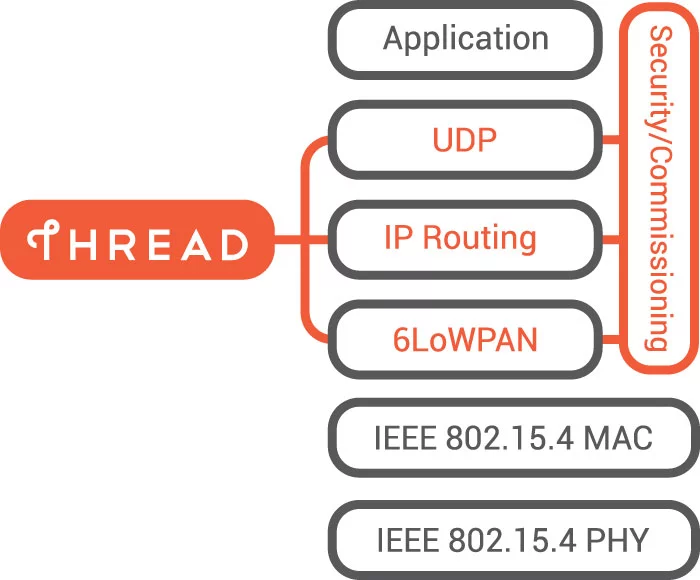
\includegraphics[width=0.5\textwidth]{images/situational_theoretical_analysis/osi_model.png}
    \caption{Thread OSI model \cite{Thread_Group_Fundamentals}.}
    \label{fig:osi_model}
\end{figure}

\subsection{Topology}
The network topology of a Thread Network depends on the number of Routers in the network. A single Router forms a basic star topology, while multiple Routers create a mesh topology, increasing reliability and redundancy. Refer to the network topology image for a visual representation of a Thread Network's basic topology, showing Routers and various device types forming a mesh network \cite{Thread_Group_Fundamentals}.

\begin{figure}[!htb]
    \centering
    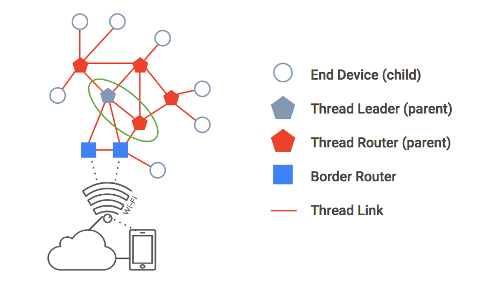
\includegraphics[width=0.8\textwidth]{images/situational_theoretical_analysis/thread_topology.png}
    \caption{Thread Network topology \cite{Thread_Group_Fundamentals}.}
    \label{fig:thread_topology}
\end{figure}

\subsection{CoAP}
CoAP (Constrained Application Protocol) is a lightweight protocol for IoT communication between constrained devices and networks, such as Thread. It enables peer-to-peer communication over IPv6 mesh networks and benefits low-power devices with limited memory. CoAP operates over UDP and offers Confirmable (CON) and Non-confirmable (NON) message types, providing flexibility in application requirements. While the maximum message size should be small enough to fit into a single packet to avoid IP fragmentation, which can increase power consumption, CoAP measurements typically focus on cases without fragmentation \cite{Lan_Thesis_Building_Automation_Systems}.

\subsection{6LoWPAN}
6LoWPAN, a protocol used by Thread devices, enables IPv6 packet transmission over IEEE 802.15.4 networks. It features header compression to minimize packet size, conserving energy and bandwidth. The mesh header improves link-layer forwarding efficiency and supports end-to-end fragmentation. Thread devices use MLE messages for node and router discovery, eliminating the need for IPv6 neighbor discovery and simplifying network operations \cite{Thread_Group_Fundamentals}.

\subsection{IEEE 802.15.4}
Thread Specification uses IEEE 802.15.4 PHY and MAC layers for link layer communication. Operating at 250 kbps in the 2.4 GHz band ensures reliable message transmission among Thread Devices. The CSMA-CA mechanism allows multiple devices to share the bandwidth while link-layer acknowledgments, retries, and security features maintain reliable and secure communication. The Thread Specification leverages the well-established IEEE 802.15.4 protocol for dependable end-to-end communication \cite{Thread_Group_Fundamentals}.

\subsection{ICMP}
ICMPv6 (Internet Control Message Protocol version 6) is integral to the IPv6 protocol suite, providing error reporting and diagnostic functions. Thread devices support ICMPv6 messages and error reporting, communicating network conditions and issues to other devices. In addition to error reporting, devices also support using echo request (ping) and echo reply messages, which are used for testing network connectivity and diagnosing network problems. With the support of ICMPv6, Thread devices can communicate and troubleshoot network issues more efficiently and streamline \cite{Thread_Group_Fundamentals}.

\subsection{No Single Point of Failure}
Thread Network is designed to operate without any single point of failure, ensuring reliable communication between devices. Devices with specific functions can be replaced automatically without disrupting communication. For instance, Sleepy End Devices automatically select another parent if their current parent is unavailable. Individual devices may lack backup capabilities in specific topologies, but the Thread Network operates autonomously to minimize the impact on users. The Leader role is dynamically elected, and if a Leader fails, another router takes its place, ensuring no single point of failure. Thus, Thread Network delivers reliable, seamless communication without depending on a single device \cite{8373620}.

\subsection{Power Consumption}
Total power consumption in Thread nodes depends on node type, radioactivity, base consumption, and application activity. Factors like functional requirements, network traffic, protocols, commissioning and maintenance logic, and environmental conditions impact radioactivity. Data transmission varies with applications sending frequent small packets or infrequent large packets, and the energy consumption is influenced by payload size. As packet size increases, transmission time and energy consumption also increase. Considering overhead added by network layers besides the actual data size is vital \cite{semiconductor_battery_2021}.


\section{Parameter Optimization}\label{sec:parameter_optimization}
Parameter optimization in wireless networks, including Thread mesh networks, balances performance and resource consumption to achieve robust and reliable networks \cite{Dave_Optimization_2006}. Fundamental techniques include adjusting transmission power, duty cycling, data rate selection, network topology and routing optimization, efficient retransmission strategies, adaptive power control, channel hopping, network scheduling, parent selection, and load balancing. These methods improve power efficiency, performance, energy consumption, battery life, and network reliability. Optimization is an iterative process that employs algorithms, simulation tools, and real-world testing to find the ideal combination of parameter values, meet performance criteria, and efficiently utilize resources \cite{butler_wifi}.

\subsection{Transmission Power}
Transmission power in Thread mesh wireless networks is vital for performance, coverage, connectivity, and power consumption. Thread operates in the 2.4 GHz ISM band based on the IEEE 802.15.4 standard, with transmission power varying due to hardware capabilities and regional regulations \cite{semiconductor_nrf52840_2018_1}. Balancing energy efficiency and network performance ensures reliable communication and minimal power consumption. Techniques for optimizing transmission power include minimum transmission power, adaptive transmission power control, and power control based on link quality, distance, traffic load, application requirements, and node energy. Additionally, multi-objective optimization and control protocols, such as Transmit Power Control, can be employed. These strategies improve energy efficiency, reduce interference, and enhance network performance.


\section{Algorithm}\label{sec:algorithm}

\subsection{Monte Carlo Method}
The Monte Carlo method is a computational technique that uses random sampling to obtain numerical results, often applied in mathematical modeling, simulation, and optimization problems across various fields such as physics, engineering, finance, and computer science.

The Monte Carlo method consists of the following steps:

\vspace{2mm}
\begin{enumerate}
    \item \textbf{Define the problem:} Identify the problem and input parameters to consider.
    \item \textbf{Generate random samples:} Produce many random samples for input parameters using random number generators or Latin hypercube sampling methods.
    \item \textbf{Run simulations:} Use each set of input parameters to simulate the problem, which could be a mathematical model or physical experiment.
    \item \textbf{Analyze the results:} Examine the simulation results to determine the system's statistical properties, including mean, variance, and standard deviation.
    \item \textbf{Refine the model:} Utilize the results to refine the model or adjust input parameters by selecting a subset of input parameters producing desirable outcomes or adjusting parameters based on statistical analysis.
    \item \textbf{Repeat:} Continue the process until a satisfactory level of accuracy is achieved.
\end{enumerate}
\vspace{3mm}

The following Monte Carlo simulation diagram shows random inputs generated and evaluated for desired results. If successful, the simulation ends; otherwise, new random inputs are developed and evaluated. This method is a powerful tool for complex problems and has widespread applications \cite{kroese2014monte}.

\begin{figure}[!htb]
    \centering
    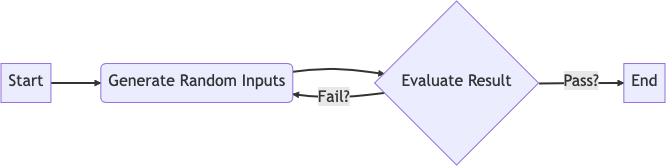
\includegraphics[width=0.8\textwidth]{images/situational_theoretical_analysis/monte_carlo_simulation.png}
    \caption{Monte Carlo Simulation diagram.}
    \label{fig:monte_carlo_simulation}
\end{figure}


\subsection{Genetic Algorithm}
Inspired by natural selection, genetic algorithms are optimization algorithms used for complex problems where traditional methods may be inefficient. They create a population of potential solutions, evaluate them based on a fitness function, and employ selection, crossover, and mutation operations to generate new solutions. Although they handle large search spaces and find global optima, limitations include random sampling, longer computation times, and potential convergence issues. Nevertheless, they are versatile engineering, finance, and machine learning tools.

The Genetic Algorithm (GA) workflow includes the following:

\vspace{2mm}
\begin{enumerate}
    \item \textbf{Initialization:} Generating a random population of potential solutions.
    \item \textbf{Selection:} Choosing the fittest individuals for the next generation.
    \item \textbf{Crossover:} Combining pairs of selected chromosomes to create offspring.
    \item \textbf{Mutation:} Introducing small random changes to offspring bit strings.
    \item \textbf{Evaluation:} Determining fitness values using a fitness function.
    \item \textbf{Termination:} Stopping the algorithm when a criterion is met.
\end{enumerate}
\vspace{3mm}

By iterating through these steps, the GA searches the solution space, converging on an optimal or near-optimal solution. A flowchart illustrates the GA's basic process, from initialization to the final solution, upon meeting a termination condition \cite{lambora2019genetic}.

\begin{figure}[!htb]
    \centering
    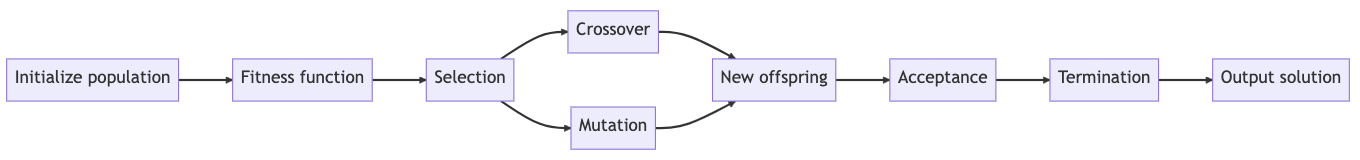
\includegraphics[width=0.8\textwidth]{images/situational_theoretical_analysis/genetic_algorithm.png}
    \caption{Genetic Algorithm flowchart.}
    \label{fig:genetic_algorithm}
\end{figure}


\section{Euclidean Distance Matrix}\label{sec:euclidean_distance_matrix}
The Euclidean distance matrix represents the straight-line distances between pairs of devices in a two-dimensional Thread network, affecting parameters like signal strength, connectivity, and energy consumption. By calculating this matrix, the research project can optimize the network using different algorithms while accounting for spatial relationships between devices.

The Euclidean distance between devices $i$ and $j$ with coordinates $(x1, y1)$ and $(x2, y2)$ is calculated as follows:

\begin{equation}\label{eq:euclidean_distance}
    distance\left(i,j\right)=\sqrt{\left(x^2-x^1\right)^2+\left(y^2-y^1\right)^2}
\end{equation}

This calculation helps account for spatial constraints and device placements, ensuring Monte Carlo random input generation considers these factors for a more efficient and optimized Thread network \cite{dokmanic2015euclidean}.

\section{RSSI Calculation}\label{sec:rssi_calculation}
Received Signal Strength Indicator (RSSI) is a vital metric in wireless systems like Thread networks, representing the received signal's power level and providing information about the wireless link quality. Antenna gains significantly influence signal strength, affecting overall performance \cite{benkic2008rssi}.

The RSSI calculation, including transmit and receive antenna gains, is:

\begin{equation}\label{eq:rssi_calculation_2}
    RSSI=P_t+G_t+G_r-L_p
\end{equation}

    Where $RSSI$ represents the Received Signal Strength Indicator $(dBm)$, $P_t$ is the transmission power $(dBm)$, $G_t$ is the transmit antenna gain $(dBi)$, $G_r$ is receive antenna gain $(dBi)$, and $L_p$ is path loss $(dB)$ \cite{doi:10.1155/2014/371350}.

\vspace{2mm}
Thread devices typically have an RSSI sensitivity of -100 dBm. This formula applies to uplink and downlink connections, offering a more accurate signal strength representation and aiding in network performance optimization and energy consumption \cite{semiconductor_nrf52840_2018_1}.

\section{General Path Loss Model}\label{sec:general_path_loss_model}
Wireless communication systems are crucial in modern life, and understanding radio wave behavior is essential for optimizing their performance. Path loss models predict received signal strength and account for gains and losses in wireless channels. This research analyzes four key path loss models and their applications in wireless communication systems.

\subsection{Free-Space Propagation Model}
The free-space propagation model is used for predicting the received signal strength in line-of-sight (LOS) environments, where there are no obstacles between the transmitter and receiver. It is often adopted for satellite communication systems. The Friis equation \ref{eq:free_space_propagation_model} describes the received power at distance $d$, considering non-isotropic antennas with transmit gain $G_t$ and receive gain $G_r$ \cite{cho2010mimo}:

\begin{equation}\label{eq:free_space_propagation_model}
    P_r\left(d\right)=\frac{P_tG_tG_r\lambda^2}{\left(4\pi\right)^2d^2L}
\end{equation}

    Where $P_t$ represents the transmit power $(watts)$, $d$ is the distance between transmitter and receiver in $meters$, $\lambda$ is the wavelength of radiation $(m)$, $G_t$ is transmit gain, $G_r$ receive gain, and $L$ is the system loss factor independent of the propagation environment. The free-space path loss ${PL}_F\left(d\right)$ can be directly derived without any system loss from \ref{eq:free_space_propagation_model}:

\begin{equation}\label{eq:free_space_path_loss}
    {PL}_F\left(d\right)\left[dB\right]=10log\left(\frac{P_t}{P_r}\right)=-10log\left(\frac{G_tG_r\lambda^2}{\left(4\pi\right)^2d^2}\right)
\end{equation}

Without antenna gains (i.e., $G_t=G_r=1$), \ref{eq:free_space_path_loss} is reduced to:

\begin{equation}\label{eq:free_space_path_loss_2}
    {PL}_F\left(d\right)\left[dB\right]=10log\left(\frac{P_t}{P_r}\right)=20log\left(\frac{4\pi d}{\lambda}\right)
\end{equation}

\subsection{Log-Distance Path Loss Model}
The log-distance path loss model is a more generalized approach, accounting for the varying path loss exponent n depending on the environment. The path loss at distance $d$ is given by \ref{eq:log_distance_path_loss_model}, where $d_0$ is the reference distance at which the path loss inherits the characteristics of free-space loss \cite{cho2010mimo}:

\begin{equation}\label{eq:log_distance_path_loss_model}
    {PL}_{LD}\left(d\right)\left[dB\right]={PL}_F\left(d_0\right)+10nlog\left(\frac{d}{d_0}\right)
\end{equation}

    Where $d_0$ is a reference distance and $n$ corresponds to free space which tends to change as shown in the table following table.

\begin{longtblr}[
  caption = {Path Loss Exponent.},
  label = {tab:path_loss_exponent},
  ]{
  colspec = {X[9cm] X[6cm]},
  hlines, vlines,
  rowhead = 1, % Repeat the header row on every page
  row{1} = {font=\bfseries},
}
  Environment & Path Loss Exponent $(n)$ \\
  Free space & 2 \\
  Urban area cellular radio & 2.7 - 3.5 \\
  Shadowed urban cellular radio & 3 - 5 \\
  In building line-of-sight & 1.6 - 1.8 \\
  Obstructed in building & 4 - 6 \\
  Obstructed in factories & 2 - 3 \\
\end{longtblr}

\vspace{2mm}
The path loss exponent $\left(n\right)$ varies based on the environment, as shown in Table \ref{tab:path_loss_exponent}, and helps to adjust the log-distance path loss model for more accurate predictions. Lower values represent environments with fewer obstructions, such as free space, while higher values indicate more complex environments with buildings or other obstacles.

\subsection{Log-Normal Shadowing Model}
The log-normal shadowing model considers the random nature of shadowing effects, making it more suitable for realistic situations. The model is given by \ref{eq:log_normal_shadowing_model}, where $X_\sigma$ is a Gaussian random variable with a zero mean and a standard deviation of $\sigma$:

\begin{equation}\label{eq:log_normal_shadowing_model}
    PL\left(d\right)\left[dB\right]=\overline{PL}\left(d\right)+X_\sigma={PL}_F\left(d_0\right)+10nlog\left(\frac{d}{d_0}\right)+X_\sigma
\end{equation}

In other words, this particular model allows the receiver at the same distance $d$ to have a different path loss, which varies with the random shadowing effect $X_\sigma$ \cite{cho2010mimo}.


\section{Literature Research}\label{sec:literature_research}
\subsection{Thread Network Power Consumption}
Thread network power consumption research has been limited but offers promising results. One study by Nordic Semiconductor demonstrates that the battery life of a Thread node is heavily dependent on the network configuration. For example, a node with an idle current of $3 \mu A$ and a transmit current of $17 mA$ can last up to 10 years in a network with a low data rate of $250 kbps$ and a small number of packets per day. However, in a network with a high data rate of $1 Mbps$ and many packets per day, the same node would only last for a few months \cite{semiconductor_battery_2021}.

In a different style, a white paper research by Thread Group provides noteworthy results on the power consumption and optimization of Thread networks. The study analyses the benefits of using a low-power wireless protocol like Thread to optimize energy consumption in Internet of Things (IoT) applications. The results of the study showed that the Thread protocol could achieve a standby power consumption of less than $3mW$, with typical transmit and receive power consumption ranging between $15mW$ and $20mW$. The study also demonstrated that devices on a Thread network could achieve up to 10 years of battery life when transmitting once per minute, making Thread a strong candidate for low-power IoT applications \cite{Thread_Low_Power_2018}.

Another research effort, conducted by Eva Azoidou at KTH Royal Institute of Technology, analyzed the power consumption of Thread end devices, routers, and coordinators. The study demonstrated that enabling power management features could reduce power consumption by up to 70\% in sleep mode. Additionally, two power optimization techniques, dynamic power management and dynamic voltage and frequency scaling, were evaluated, with the latter having a greater impact, reducing consumption by up to 35\%. The research also emphasized that power consumption is influenced by transmission power level, data rate, and routing topology and suggested that implementing optimization techniques could reduce power consumption by up to 70\% \cite{azoidou2017battery}.

In summary, although the literature on Thread power optimization is limited, the results from existing studies suggest that the protocol has significant potential for reducing energy consumption in low-power wireless networking applications. More research is needed to fully understand and optimize the power consumption of Thread networks in large-scale deployments.


\section{Algorithm}\label{sec:algorithm_research}
\subsection{Monte Carlo Method}
The Monte Carlo method (MCM) is a robust, efficient, flexible, and scalable tool used across various fields, including science, finance, and engineering. Research by Kroese emphasizes MCM's popularity and its applications in areas like industrial engineering, operations research, physical processes, random graphs, finance, biology, medicine, and computer science. The authors highlight MCM's simplicity, strength in randomness, and theoretical justification \cite{kroese2014monte}.

In contrast, William Oberle's technical note from the US Army Research Laboratory discusses the number of iterations required for accurate estimation and the accuracy or error in estimating of the probability distribution's mean. The research emphasizes the relationship between these topics through the central limit theorem and provides methods for estimating the number of iterations and confidence intervals. The study also highlights the importance of caution when dealing with small sample sizes or non-normal distributions \cite{oberle2015monte}.

Overall, MCM has significantly influenced quantitative problem-solving across numerous research fields, becoming an indispensable tool for understanding complex systems.

\subsection{Genetic Algorithm}
Genetic Algorithm (GA) is a heuristic optimization algorithm that handles non-linear, non-convex, and intermittent problems. It is widely applied in various engineering and scientific applications.

One study employs GA to optimize wireless sensor networks (WSNs) for precision agriculture applications. The research determines active sensors, cluster heads, and signal ranges while considering network connectivity, energy conservation, and application requirements. Results indicate that GA-generated designs outperform random deployments regarding connectivity and energy consumption \cite{ferentinos2005energy}.

In another research, Norouzi and Zaim explores the potential of GA in optimizing the operational stages of WSNs. The authors discuss node placement, network coverage, clustering, data aggregation, and routing. Simulations demonstrate that GA-based approaches outperform existing protocols, suggesting that GA can optimize WSNs in military, medical, and commercial applications \cite{norouzi2014genetic}.

Lastly, a research survey explores GA applications, insights, and future directions in wireless networking. It addresses key challenges such as parameter selection, enhancing theoretical understanding, and developing efficient multi-objective GAs. The survey emphasizes the need for further research to address open issues and explore new applications in wireless networking \cite{mehboob2016genetic}.

In summary, GA is a powerful tool for optimizing parameters in various applications. However, its computational complexity increases with the number of parameters, making it challenging to apply to large-scale problems.


\section{Hardware Analysis}\label{sec:hardware_analysis}
\subsection{nRF52840 DK}
The nRF52840 DK by Nordic Semiconductor is a versatile IoT and wireless connectivity development kit featuring a 32-bit ARM Cortex-M4F processor, $1MB$ flash memory, and $256KB$ RAM. The kit supports protocols like Bluetooth 5, Mesh, Thread, and Zigbee. The kit includes an onboard debugger, external antenna, sensors, and peripherals. Compatible with software tools like nRF5 SDK, nRF Connect SDK, and Zephyr RTOS, it offers multiple SoC support, Bluetooth 5.3 multiprotocol radio, Arduino Rev3 shield compatibility, onboard programming/debugging, direct USB interface, external memory support, integrated antennas, SWF RF connector, user-programmable buttons and LEDs, and various power supply options, making it ideal for low-power, high-performance wireless applications \cite{Semiconductor_Nordic_Product_Brief_2018_2.0}.

\begin{figure}[!htb]
    \centering
    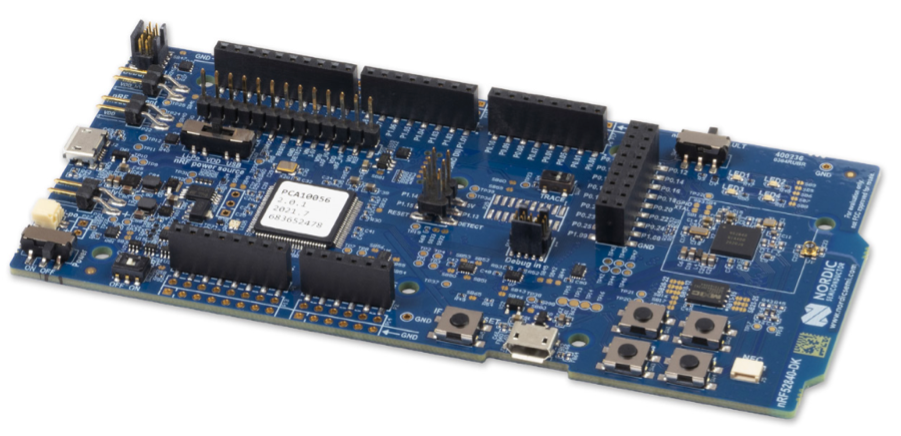
\includegraphics[width=0.5\textwidth]{images/situational_theoretical_analysis/nRF52840_DK.png}
    \caption{Nordic Semiconductor nRF52840 DK \cite{Semiconductor_Nordic_Product_Brief_2018_2.0}.}
    \label{fig:nRF52840_DK}
\end{figure}

\subsection{nRF52840 Dongle}
The nRF52840 Dongle by Nordic Semiconductor is a compact, cost-effective platform for wireless application development, offering multiprotocol radio, Bluetooth 5.2 readiness, IEEE 802.15.4 radio, Thread, and Zigbee support. Featuring an Arm Cortex-M4 processor, DSP instruction set, and enhanced security through the Arm CryptoCell CC310 cryptographic accelerator, the dongle includes 15 accessible GPIOs, a direct USB interface, and an integrated 2.4 GHz PCB antenna. It also has one user-programmable button, one user-programmable RGB LED, and one additional programmable LED. The device operates between 1.7 and 5.5 V, powered via USB or external sources \cite{Semiconductor_Nordic_Dongle_Brief_2018_2.0}.

\begin{figure}[!htb]
    \centering
    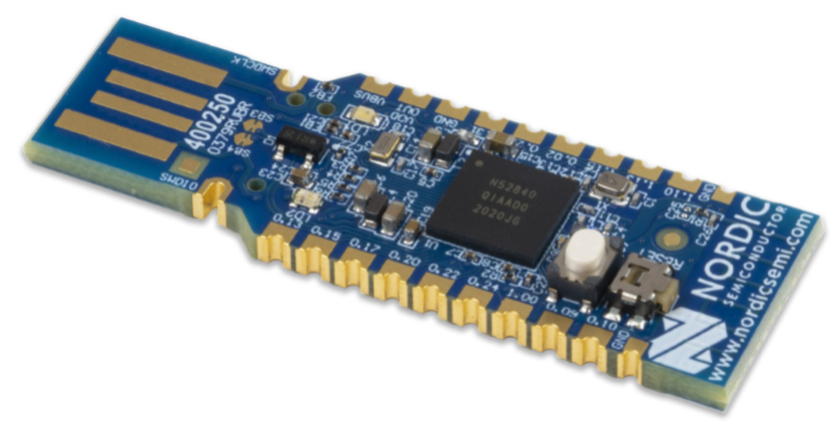
\includegraphics[width=0.5\textwidth]{images/situational_theoretical_analysis/nRF52840_Dongle.png}
    \caption{Nordic Semiconductor nRF52840 Dongle \cite{Semiconductor_Nordic_Dongle_Brief_2018_2.0}.}
    \label{fig:nRF52840_Dongle}
\end{figure}

\subsection{Power Profiler Kit II}
The nRF Power Profiler Kit II (nRF PPK II) is a precise power profiler for optimizing power consumption in embedded systems using Nordic Semiconductor's nRF5x and nRF91 Series devices. It provides high accuracy with a resolution of up to 140 nA and a dynamic range of 100 mA to 1 A, allowing developers to correlate power consumption with code execution, measure real-time power consumption, and optimize battery life. Key features include a wide current measurement range, source and ampere meter modes, a programmable regulator, a high sampling rate of up to 100 kbps, compatibility with all Nordic DKs and custom boards, and support for nRF Connect for Desktop's Power Profiler app. The nRF PPK II is ideal for engineers seeking a comprehensive, flexible, and user-friendly power profiling tool \cite{Semiconductor_Nordic_PPK_II_2018_1.0}.

\begin{figure}[!htb]
    \centering
    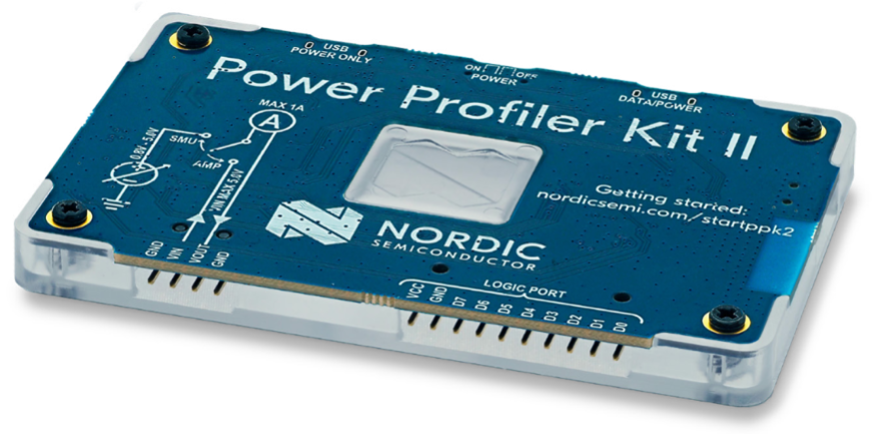
\includegraphics[width=0.3\textwidth]{images/situational_theoretical_analysis/nRF_Power_Profiler_Kit_II.png}
    \caption{Nordic Semiconductor nRF Power Profiler Kit II \cite{Semiconductor_Nordic_PPK_II_2018_1.0}.}
    \label{fig:nRF_Power_Profiler_Kit_II}
\end{figure}

\subsection{Raspberry Pi}
The Raspberry Pi 4 is a popular, low-cost single-board computer with versatile capabilities. It can function as a Thread border router when paired with an nRF DK or Dongle that supports Thread. Thread is a low-power, wireless mesh networking protocol designed for IoT devices. The nRF DK or Dongle is the Thread radio, enabling communication between the Raspberry Pi and Thread-enabled devices. This combination offers an affordable, easy-to-use, and versatile solution for building a Thread border router. The Raspberry Pi 4's general-purpose computing capabilities allow it to host various applications for managing and monitoring the network \cite{alm2019internet}.

\begin{figure}[!htb]
    \centering
    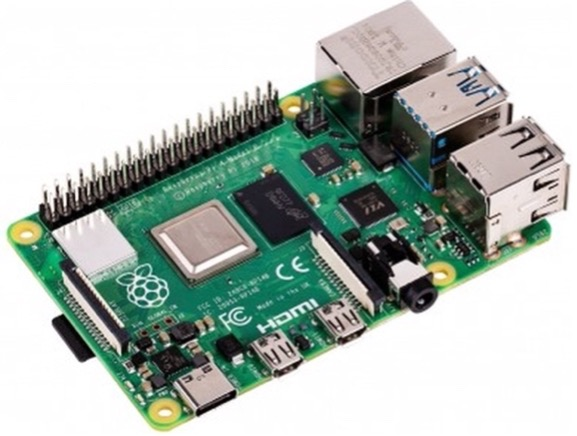
\includegraphics[width=0.5\textwidth]{images/situational_theoretical_analysis/Raspberry_Pi_4.jpg}
    \caption{Raspberry Pi 4 \cite{Pi_Raspberry_Pi_4_Model_B_2019_1.0}.}
    \label{fig:Raspberry_Pi_4}
\end{figure}
